\documentclass[12pt, a4paper, oneside]{Thesis} % Paper size, default font size and one-sided paper
\usepackage{wrapfig}
\usepackage{lscape}
\usepackage{rotating}
\usepackage{graphicx}
\usepackage{caption}
\usepackage{amsmath}


\usepackage{lineno,hyperref}
\modulolinenumbers[5]

\usepackage{caption}
\usepackage{subcaption}
\usepackage{algorithm}% http://ctan.org/pkg/algorithms
\usepackage{algpseudocode}
\usepackage{algorithmicx}

\usepackage{amssymb}
\usepackage{graphicx}
\usepackage{array}
\usepackage{float}
\usepackage{placeins}
\usepackage{stackengine}
\usepackage{url}
\usepackage{numprint}
\usepackage{caption}

\usepackage{booktabs}
\usepackage{siunitx}
%\usepackage[showframe=false]{geometry}
\usepackage{subfigure}

\nprounddigits{3}
\newcolumntype{P}[1]{>{\centering\arraybackslash}p{#1}}
\newcolumntype{M}[1]{>{\centering\arraybackslash}m{#1}}

\setstackEOL{\#}
\setstackgap{L}{12pt}


%\usepackage{subcaption} %incompatible with subfig
\graphicspath{{Pictures/}} % Specifies the directory where pictures are stored
\usepackage{natbib} % Use the natbib reference package - read up on this to edit the reference style; if you want text (e.g. Smith et al., 2012) for the in-text references (instead of numbers), remove 'numbers' v

\hypersetup{urlcolor=black, colorlinks=false} % Colors hyperlinks in blue - change to black if annoyingv`	

\thesistitle{Smart Fall Detection System}
\supervisor{Professor Sudip Misra}
\degree{Bachelor of Technology}
\degreemajor{Computer Science and Engineering}
\authors{Adhithya and Tejaraam}
\rollno{22CS30019 and 22CS30059}
\university{Indian Institute of Technology Kharagpur}
\department{Department of Computer Science and Engineering}
\unisite{http://www.iitkgp.ac.in/}
\depsite{http://cse.iitkgp.ac.in/}
\placeshrt{Kharagpur}
\placelng{Kharagpur - 721302, India}
\datesub{11th November 2025}
\datesig{11th November 2025}
\semsub{Autumn Semester, 2025-26}
\keywords{Wearable Sensor, Accelerometer, Gyroscope, Machine Learning, Random Forest, IoT, Fall Detection}

\title{\ttitle} % Defines the thesis title - don't touch this
\begin{document}
%\makeatletter
%\renewcommand*{\NAT@nmfmt}[1]{\textsc{#1}}
%\makeatother

% prints author names as small caps


\frontmatter % Use roman page numbering style (i, ii, iii, iv...) for the pre-content pages

\setstretch{1.6} % Line spacing of 1.6 (double line spacing)

% Define the page headers using the FancyHdr package and set up for one-sided printing
\fancyhead{} % Clears all page headers and footers
\rhead{\thepage} % Sets the right side header to show the page number
\lhead{} % Clears the left side page header

%\pagestyle{fancy} % Finally, use the "fancy" page style to implement the FancyHdr headers

\newcommand{\HRule}{\rule{\linewidth}{0.5mm}} % New command to make the lines in the title page

% PDF meta-data
\hypersetup{pdftitle={\ttitle}}
\hypersetup{pdfsubject=\subjectname}
\hypersetup{pdfauthor=\authornames}
\hypersetup{pdfkeywords=\keywordnames}

%----------------------------------------------------------------------------------------
%	TITLE PAGE
%----------------------------------------------------------------------------------------
\coursecd{CS61066} % Define your course code here
\maketitle
%\titlepg % Add a gap in the Contents for aesthetics

\clearpage % Start a new page

%----------------------------------------------------------------------------------------
%	DECLARATION PAGE (UNCOMMENTED)
%----------------------------------------------------------------------------------------


\Declaration% Add a gap in the Contents for aesthetics


%----------------------------------------------------------------------------------------
%	CERTIFICATE PAGE (UNCOMMENTED)
%----------------------------------------------------------------------------------------

\addtotoc{Certificate} % Add the "Abstract" page entry to the Contents

\certificate{\addtocontents{toc}{} % Add a gap in the Contents, for aesthetics

\clearpage % Start a new page

%----------------------------------------------------------------------------------------
%	ABSTRACT PAGE (UNCOMMENTED AND FILLED)
%----------------------------------------------------------------------------------------

\addtotoc{Abstract} % Add the "Abstract" page entry to the Contents

\abstract{\addtocontents{toc}{} % Add a gap in the Contents, for aesthetics

A Fall-Detection Device basically monitors the accelerometer and gyropscope readings of the person to which it was attached and tries to identify the fall pattern from the statistical data, which it derives from the sensor data. For analysing those, we will use a trained ML model deployed in the cloud. This device is not only capable of finding the fall patterns, but it can also collect the movement data in terms of statistical features of accelerometer and gyroscopic readings for future use, which can be further used to train the deployed model after labelling.

The Device was intended to be multi-tasking. The device has two different modes, namely Data-Collection Mode, Data-Prediction Mode, for serving two unique functionalities. Data-Collection Mode: Our Device will collect the data from the sensors and compute the statistical features like mean, max, min and variance for each of the 6 sensor parameters [ ax,ay,az,gx,gy,gz] and send to the backend server to store for future labelling purposes. Data-Prediction Mode: Uses the trained ML model deployed in the cloud for real-time fall prediction.

\textbf{\textit{Keywords - }} Wearable Sensor, Accelerometer, Gyroscope, Machine Learning, Random Forest, IoT, Fall Detection
}

\clearpage % Start a new page



%----------------------------------------------------------------------------------------
%	ACKNOWLEDGEMENTS (UNCOMMENTED)
%----------------------------------------------------------------------------------------

\setstretch{1.3} % Reset the line-spacing to 1.3 for body text (if it has changed)

{\addtocontents{toc}{}} % Add a gap in the Contents, for aesthetics
\chapter*{Acknowledgement}

I would like to express my sincere gratitude to my supervisor, Prof. Sudip Misra, for his constant guidance, valuable suggestions, and encouragement throughout this project.  
I am also thankful to our teaching assistant, Mr. Biswajit Ghosh, for his support and helpful feedback during the development of this work.  

I would like to thank my friends and family for their continuous motivation, patience, and support, which helped me complete this project successfully.

% }
\clearpage % Start a new page


%----------------------------------------------------------------------------------------
%	LIST OF CONTENTS/FIGURES/TABLES PAGES (UNCOMMENTED)
%----------------------------------------------------------------------------------------

\pagestyle{fancy} % The page style headers have been "empty" all this time, now use the "fancy" headers as defined before to bring them back

\lhead{\emph{Contents}} % Set the left side page header to "Contents"
\tableofcontents % Write out the Table of Contents

\lhead{\emph{List of Figures}} % Set the left side page header to "List of Figures"
\listoffigures % Write out the List of Figures

\lhead{\emph{List of Tables}} % Set the left side page header to "List of Tables"
\listoftables % Write out the List of Tables

%----------------------------------------------------------------------------------------
%	ABBREVIATIONS (UNCOMMENTED AND FILLED)
%----------------------------------------------------------------------------------------

\clearpage % Start a new page

\setstretch{1.5} % Set the line spacing to 1.5, this makes the following tables easier to read

\lhead{\emph{Abbreviations}} % Set the left side page header to "Abbreviations"
\listofsymbols{ll} % Include a list of Abbreviations (a table of two columns)
{

\textbf{ML} & \textbf{M}achine \textbf{L}earning \\
\textbf{IoT} & \textbf{I}nternet \textbf{o}f \textbf{T}hings \\
\textbf{RF} & \textbf{R}andom \textbf{F}orest \\
\textbf{XGBoost} & E\textbf{x}treme \textbf{G}radient \textbf{B}oosting \\

}


%----------------------------------------------------------------------------------------
%	THESIS CONTENT - CHAPTERS
%----------------------------------------------------------------------------------------

\mainmatter % Begin numeric (1,2,3...) page numbering

\pagestyle{fancy} % Return the page headers back to the "fancy" style

% Include the chapters of the thesis as separate files from the Chapters folder
% Uncomment the lines as you write the chapters

% Chapter Template

\chapter{Introduction} % Main chapter title

\label{Chapter 1} % Change X to a consecutive number; for referencing this chapter elsewhere, use \ref{ChapterX}

\lhead{Introduction } % Change X to a consecutive number; this is for the header on each page - perhaps a shortened title

\section{Introduction}
A Fall-Detection Device basically monitors the accelerometer and gyropscope readings of the person to which it was attached and tries to identify the fall pattern from the statistical data, which it derives from the sensor data. For analysing those, we will use a trained ML model deployed in the cloud . This device is not only capable of finding the fall patterns, but it can also collect the movement data in terms of statistical features of accelerometer and gyroscopic readings for futur usee, which can be further used to train the deployed model after labelling

\section{Motivation}
Many Elderly people will die due to unexpected fall accidents, to make sure we have continuous monitoring of the movement, what if we have a device that analyses the movement patterns, continuously identifies the fall accidents immediately within a fraction of second, alerting the caretakers.  

\section{Contribution of Project}
This project was made into three different sections Frontend, Backend and Hardware. 

The Frontend and hardware sections are looked after by the V.Tejaraam which includes creation of visually appealing dashboard and interactive labeling page along with hardware simulation and connection.

The system architecture and backend server design along with model creation was looked after by D.Adhithya, he design the endpoints, end to end communication and model for identifying the fall pattern, all the connectivity issues, debugging, logs and managing database was covered in the backend server design itself.  

\chapter{Literature Review} % Main chapter title

\label{Chapter 2}

\lhead{Literature Review} % Change X to a consecutive number; The transition of Computer Numerical Control (CNC) systems into the Industry 4.0 era has necessitated a shift from isolated, rigid hardware configurations toward interconnected, intelligent ecosystems. This chapter explores the convergence of Predictive Maintenance (PdM) and advanced CAD/CAM methodologies, tracing the evolution from traditional statistical models to modern Deep Learning (DL) and cloud-integrated frameworks.

\section{Evolution of Predictive Maintenance (PdM) Models}
Early research in CNC maintenance was primarily concerned with establishing a theoretical foundation for algorithm selection. \cite{cinar2020mlpdm} utilized the PRISMA taxonomy to categorize the burgeoning landscape of Machine Learning (ML) techniques, identifying a persistent gap between theoretical model performance and actual shop-floor deployment. As manufacturing moved toward the cloud, \cite{paolanti2018mlindustry4} demonstrated the feasibility of using Random Forest (RF) architectures within Azure for motor downtime prediction, though these early models were often limited by their simplicity. 

Recent studies have focused on increasing the granularity and interpretability of these models. \cite{wakhare2023optimizing} compared RF, Gradient Boosting, and Neural Networks to provide a more transparent model selection process specifically for CNC interpretability. However, as noted by \cite{sarikaya2024predictive}, the challenge for Small and Medium Enterprises (SMEs) remains the digitization of historical data to feed these complex algorithms.


\begin{table}[H]
\centering
\caption{State-of-the-Art Literature Summary}
\label{tab:litreview}
\resizebox{\textwidth}{!}{%
\begin{tabular}{|p{3cm}|p{1.5cm}|p{2cm}|p{3cm}|p{3cm}|p{2cm}|}
\hline
\textbf{Paper} & \textbf{Year} & \textbf{Method} & \textbf{Problem} & \textbf{Gap} & \textbf{Relevance} \\
\hline
\cite{luo2020hybrid} & 2020 & Digital Twin+data-driven & Lifecycle inconsistency & Heavy DT & Cloud PdM baseline \\
\hline
\cite{srivastava2023stepnc} & 2023 & STEP-NC review & G-code bottleneck & No empirical & CAD-CNC integration \\
\hline
\cite{cinar2020mlpdm} & 2020 & PRISMA taxonomy & ML selection & Theoretical & PdM landscape \\
\hline
\cite{paolanti2018mlindustry4} & 2018 & RF Azure & Downtime motors & Simple ML & Cloud RF \\
\hline
\cite{wakhare2023optimizing} & 2023 & RF/GB/NN & Interpretability & CNC-specific & Model comparison \\
\hline
\cite{toquica2019stepncrobot} & 2019 & STEP-NC robots & Interoperability & G-code translation & CNC arch \\
\hline
\cite{sarikaya2024predictive} & 2024 & LSTM/GRU & SME digitization & Historical data & RUL forecasting \\
\hline
\cite{zhang2025camaservice} & 2025 & NSGAIII-CaaS & Toolpath flexibility & Human strategy & Cloud CAM \\
\hline
\cite{arjun2025predictive} & 2025 & RF/LSTM & Interpretability & Single platform & Multimodal \\
\hline
\cite{thoppil2025iiot} & 2025 & LSTM IIoT & Offline analysis & Spindle only & Real-time spindle \\
\hline
\cite{sridevi2025predictive} & 2025 & RF Arduino & Reactive maint & RUL regression & Lightweight \\
\hline
\cite{pu2026deeplearning} & 2026 & CNN-LSTM & Nonlinear degradation & Black-box & DL fusion \\
\hline
\end{tabular}%
}
\end{table}

This review highlights need for integrated PdM+CAD/CAM our system addresses.

 
% ================================
% Chapter: System Methodology
% ================================

\chapter{System Methodology}
\label{Chapter3}
\lhead{System Methodology}

\section{System Components and Architecture}

The PdM system uses multi-layer IIoT architecture for CNC monitoring: sensors → edge processing → cloud ML → dashboard.

\vspace{0.5cm}

\begin{figure}[H]
    \centering
    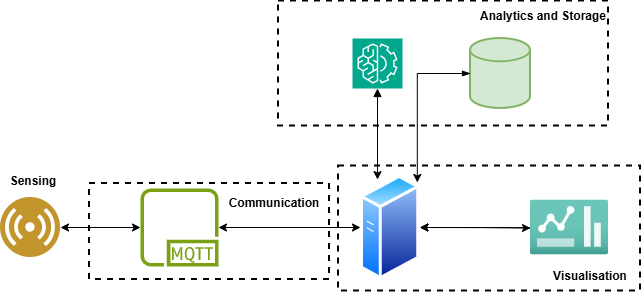
\includegraphics[width=0.8\textwidth, height=0.4\textheight, keepaspectratio]{arch.png}
    \caption{Overall IIoT Architecture for CNC PdM (suggest: add cnc\_arch\_placeholder.png for detailed CAD-CNC flow)}
    \label{fig:arch}
\end{figure}

\newpage

\begin{table}[H]
    \centering
    \caption{IIoT System Layers and Components}
    \label{tab:iot_layers}
    \renewcommand{\arraystretch}{1.0}
    \setlength{\tabcolsep}{4pt}
    \resizebox{\textwidth}{!}{
    \begin{tabular}{|m{2.8cm}|m{3.5cm}|m{8.2cm}|}
        \hline
        \textbf{Layer} & \textbf{Components} & \textbf{Description} \\
        \hline
        Sensing & MPU6050/Vib/Temp & CNC sensors (vibration, temp, acoustics). \\
        \hline
        Edge & ESP32 & Computes features (mean, var, FFT) for 6+ axes. \\
        \hline
        Comm & WiFi/MQTT & Power-efficient to Flask backend. \\
        \hline
        Analytics & RF/LSTM models & PdM classification/RUL (saved\_models/). \\
        \hline
        App & React Dashboard & Live feed, labeling, retrain (cnc\_automation\_project). \\
        \hline
    \end{tabular}
    }
\end{table}

\vspace{0.5cm}

\begin{figure}[H]
    \centering
    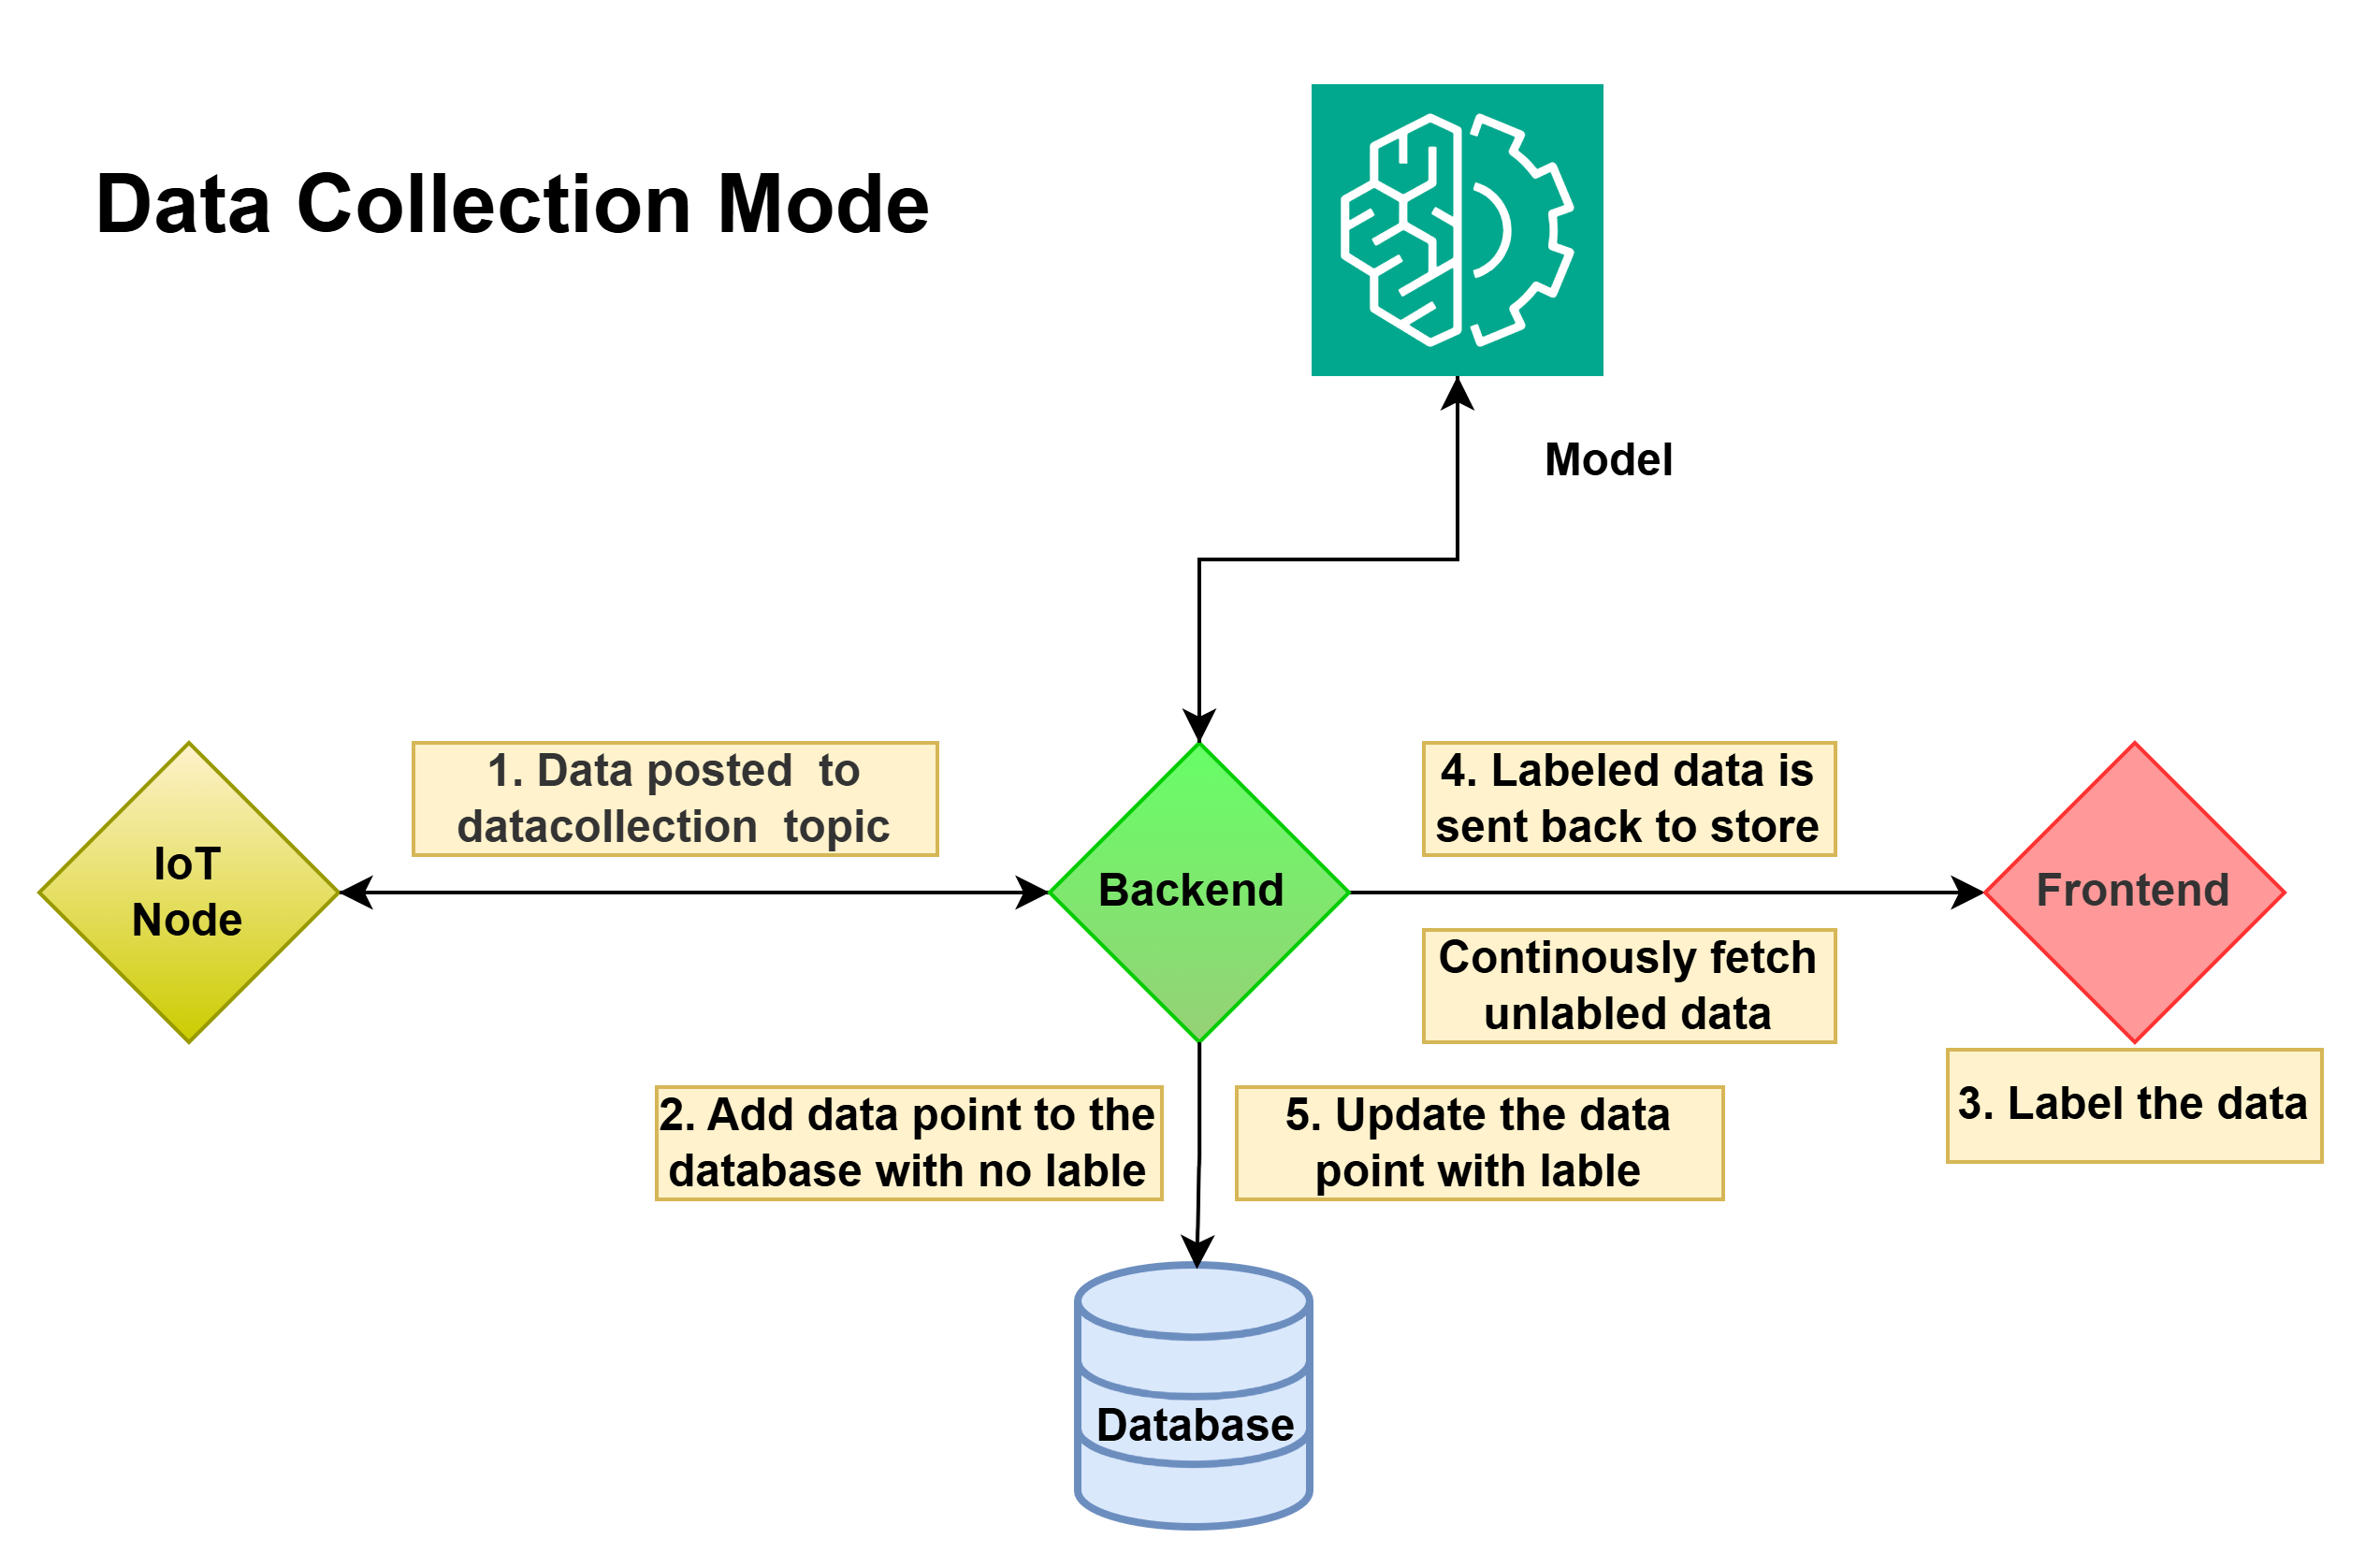
\includegraphics[width=0.8\textwidth, height=0.3\textheight, keepaspectratio]{collection.png}
    \caption{Data Collection Mode (suggest: sensor\_data\_placeholder.png)}
\end{figure}

\newpage

\begin{figure}[H]
    \centering
    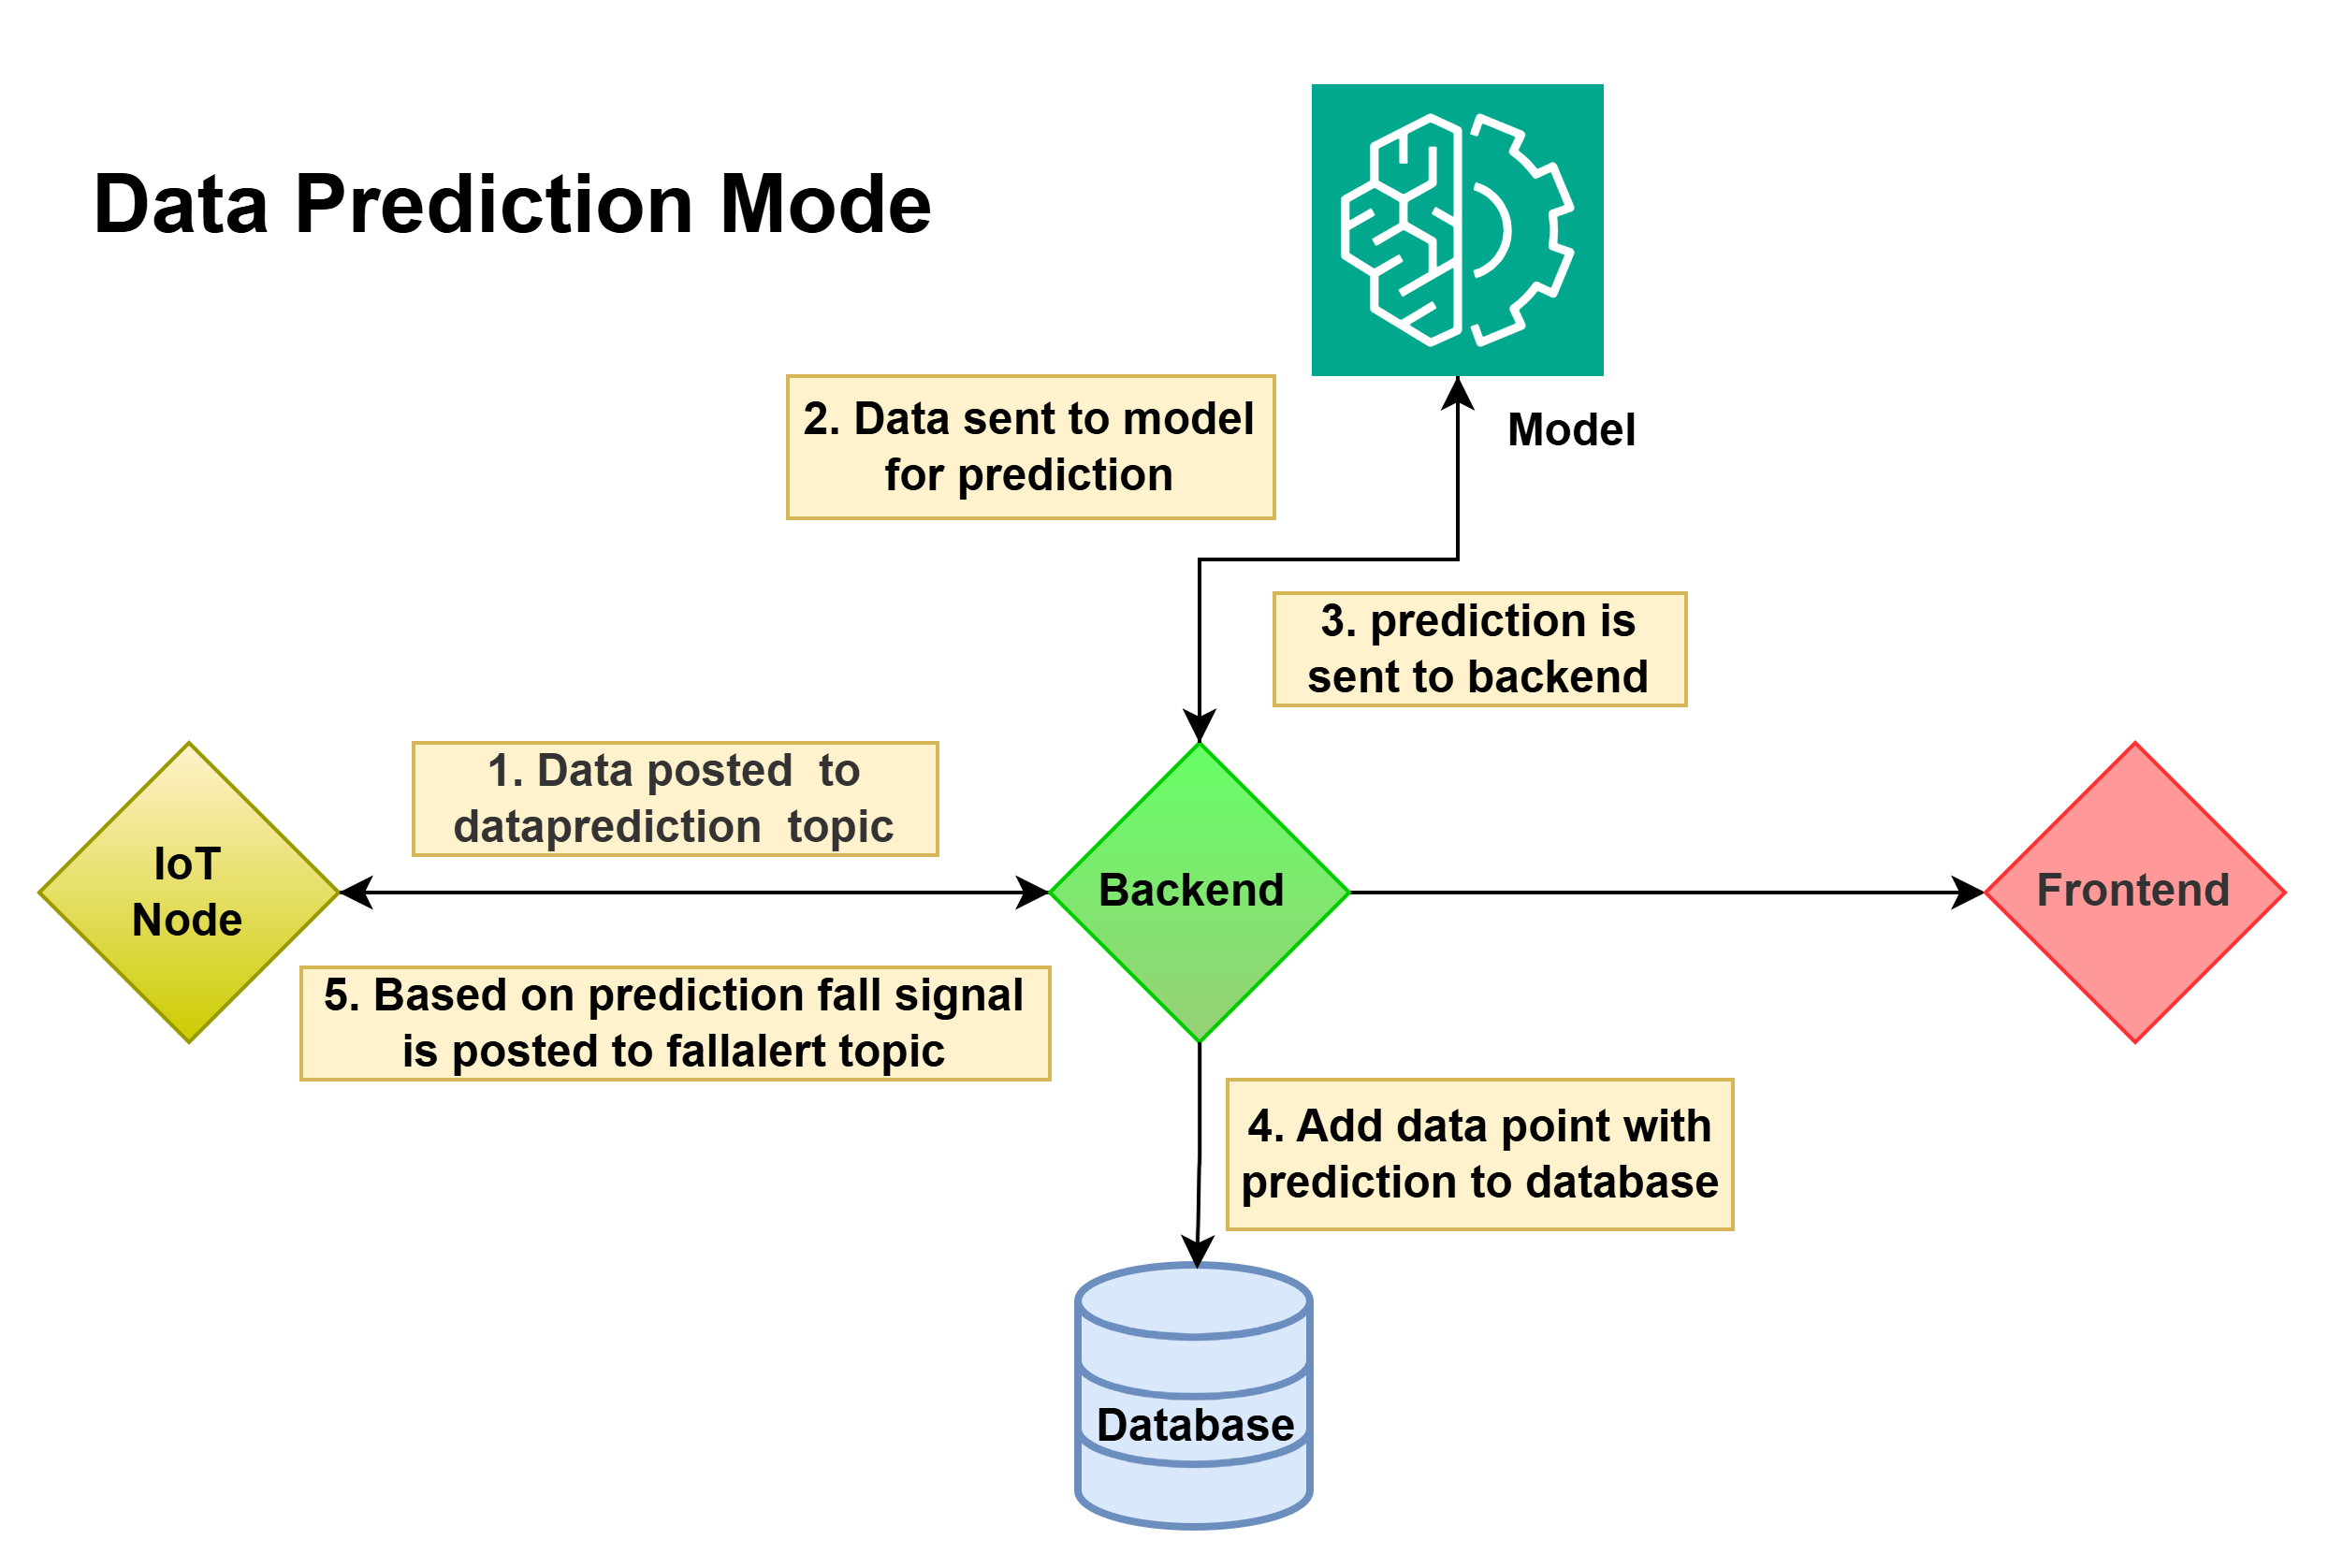
\includegraphics[width=0.8\textwidth, height=0.4\textheight, keepaspectratio]{prediction.png}
    \caption{PdM Prediction Mode (suggest: pdm\_plot\_placeholder.png)}

    \vspace{0.7cm}

    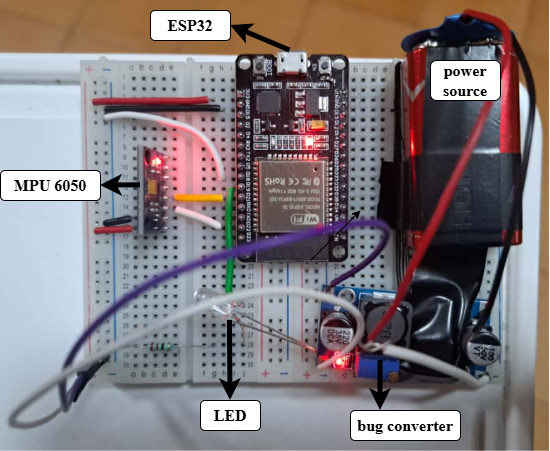
\includegraphics[width=0.8\textwidth, height=0.4\textheight, keepaspectratio]{hardware.png}
    \caption{CNC Sensor Hardware Setup (suggest: cnc\_hardware\_placeholder.png)}
\end{figure}

\newpage

\begin{figure}[H]
    \centering
    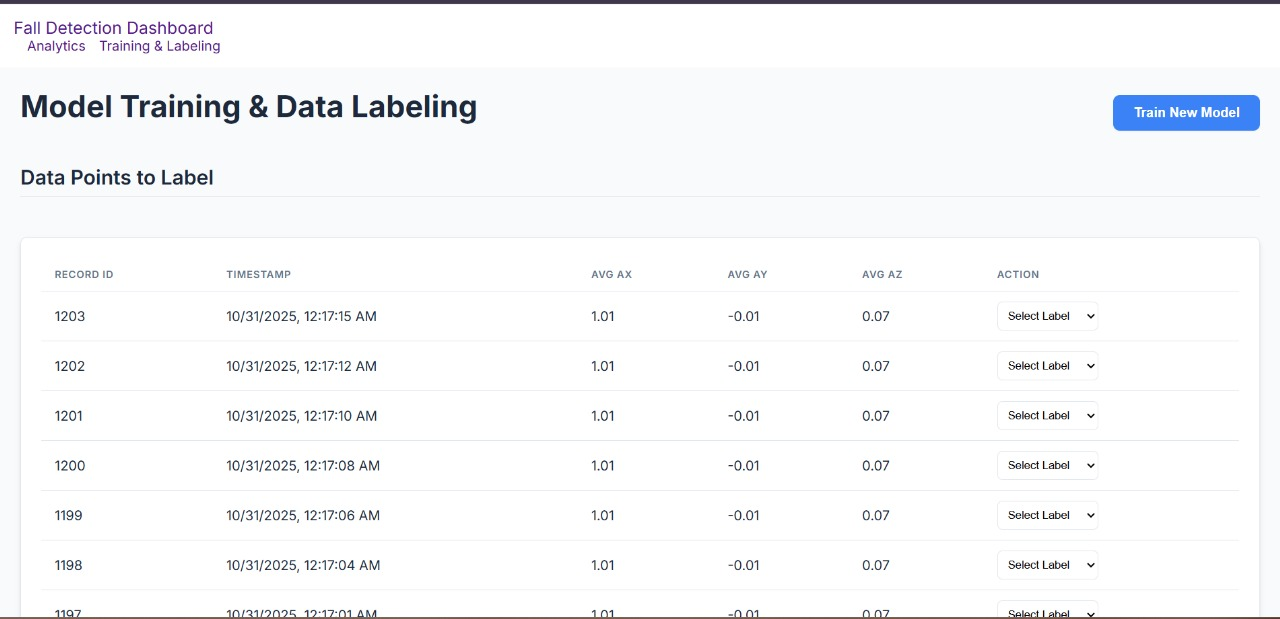
\includegraphics[width=1\textwidth, height=0.7\textheight, keepaspectratio]{ui.jpg}
    \caption{Frontend Dashboard — Labeling (Machine Health page)}

    \vspace{0.7cm}

    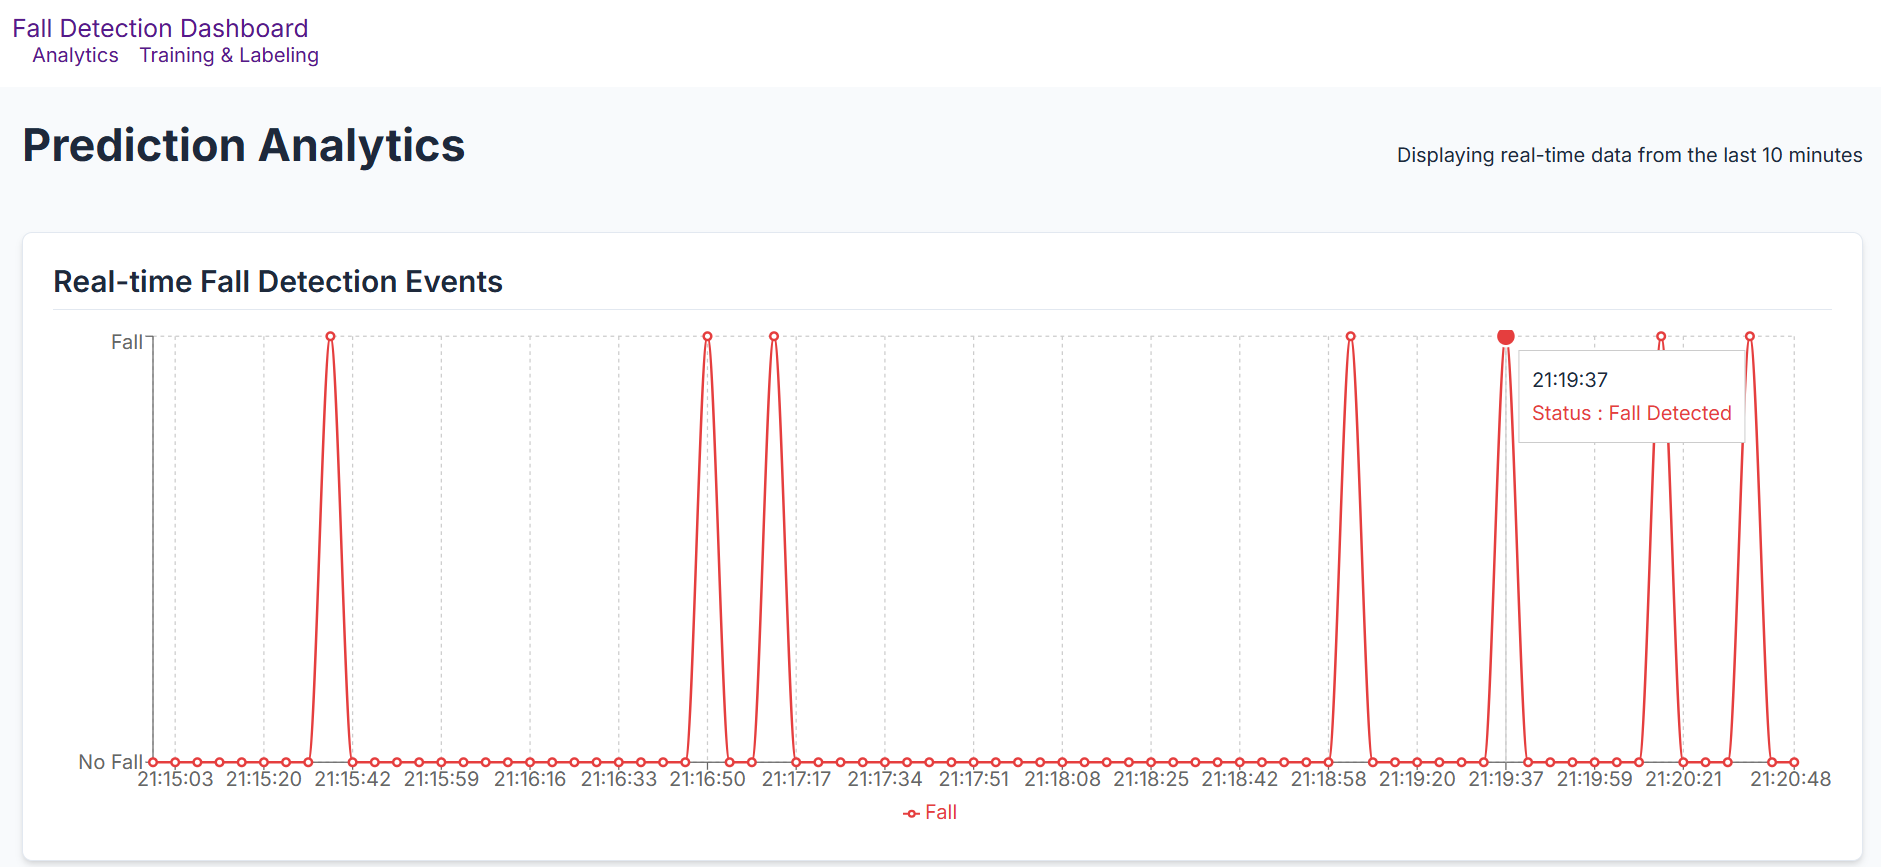
\includegraphics[width=1\textwidth, height=0.7\textheight, keepaspectratio]{analytics.png}
    \caption{Analytics View (Health predictions)}
\end{figure}

 
% ================================
% Chapter: Experimental Setup
% ================================

\chapter{Experimental Setup}
\label{Chapter4}
\lhead{Experimental Setup}

\section{Dataset Preparation}

\subsection{Custom Data Collection}
Initially we used sisfall dataset but the sensor used to create this dataset is not same as our sensor.
So we manually collect the data and labelled the data with our sensor.

We need to tag fall or nofall manually for every datapoint and initial most of the times when experiment is conducted if we connected module with battery , battery used to get disconnected so we connected usb to the ESP32 and collected the data.

\subsection{Selection of ML Model}
Since our dataset was prepared manually due to constrain of resources we are only able to collect 1000 datapoints, so due to lack of knowledge about different models performance on small dataset we were not able to prioritise which model to use initially.
So we trained regression model, decision tree, random forest, Xg boost, neural network models and decided based on the accuracy of model.

\subsection{Hardware Setup}
The hardware device we have designed typically contains four different sections.

Power Source :  We have used a 9V battery and a LM2596 Buck convertor to step down to the 3.3V power supply.

MPU6050 Sensor: This is the Sensor which collects the accelerometer and Gyroscopic data of the person ,it send the data from the SDA and SCL to the D21 and D22 Pins of the ESP32.

ESP32 Microcontroller: This is the Central Processing Unit of the hardware device ,which collects the sensor data processes it and determine where to post based on the input signal from the MODE Pin which is D18,and also on receiving the alertsignal   on the ‘fallalert’ topics it will make the D19 pin high to actuate LED.

Actuator (LED) : we have used an LED light for actuation ,Whenever there is a fall detected it will be actuated by ESP32.
 
\chapter{Challenges} % Main chapter title

\label{Chapter 5} % Change X to a consecutive number; for referencing this chapter elsewhere, use \ref{ChapterX}

\lhead{Results and Observation }

\section{Results}

 
\chapter{Conclusion and Further Work} % Main chapter title
\label{Chapter 6}


\lhead{Conclusion and Further Work }

\section{Conclusion}
In conclusion, the Fall-Detection Device helps keep track of a person’s movements using data from the accelerometer and gyroscope. It can quickly find out if a fall has happened by using a trained machine learning model stored in the cloud. Along with detecting falls, the device also saves movement data in the form of useful numbers. This data can later be labelled and used to retrain the model, making the system smarter and more accurate over time.

\section{Future Work}
Future work involves addressing the challenges identified in the current system, specifically:
\begin{enumerate}
    \item Enhancing stability and robustness of the system while running entirely on a battery unit for long time, like using batteries which can charge.

    \item Collecting a larger, more diverse dataset to train more robust ML models.
    \item As this is a prototype we actuated using led, insted we can send this actuation signal as notification to caretaker's mobile.
\end{enumerate} 

%----------------------------------------------------------------------------------------
%	THESIS CONTENT - APPENDICES
%----------------------------------------------------------------------------------------

\addtocontents{toc}{\vspace{2em}} % Add a gap in the Contents, for aesthetics

\appendix % Cue to tell LaTeX that the following 'chapters' are Appendices

% Include the appendices of the thesis as separate files from the Appendices folder
% Uncomment the lines as you write the Appendices

% \input{Appendices/AppendixA}
%\input{Appendices/AppendixB}
%\input{Appendices/AppendixC}

\addtocontents{toc}{} % Add a gap in the Contents, for aesthetics

\backmatter

%----------------------------------------------------------------------------------------
%	BIBLIOGRAPHY (UNCOMMENTED)
%----------------------------------------------------------------------------------------
%\nocite{*}
\label{Bibliography}

\lhead{\emph{Bibliography}} % Change the page header to say "Bibliography"

\bibliographystyle{apalike} % Use the "custom" BibTeX style for formatting the Bibliography

\bibliography{Bibliography} % The references (bibliography) information are stored in the file named "Bibliography.bib"

\end{document}